	\subsection{Sposób filtracji}
Do danych zbieranych w projekcie często dojdą takie, które mogą zaburzyć otrzymanie prawidłowego wyniku. Jedną z metod, aby poradzić sobie z tym jest filtracja danych poprzez odrzucenie tych najbardziej skrajnych. Danych mozna odrzucić nawet połowę próbek, aczkolwiek przypadek przedstawiony tutaj nie potzrebuje aż tak rygorystycznych reguł. Dane, które odrzucimy to będą 3 próbki osób, które po prostu zawyżyły cenę swoich mieszkań. Ważnym jest, żeby przefiltrować dane w odpowiedni sposób odrzucając te próbki, które mogą mieć najbardziej negatywny wpływ na wynik końcowy.
	\subsection{Odrzucenie danych}
Skoro celem naszego algorytmu jest znalezienie zależności między ceną mieszkania, a jego metrażem, możemy stwierdzić w uproszczeniu, że poszukujemy tak naprawdę średniej ceny za metr kwadratowy mieszkania we Wrocławiu.
\newline
\newline
\noindent
\(
	y  \hspace{2.1cm} \textrm{cena mieszkania} [zl] \\
	X  \hspace{2cm} \textrm{powierzchnia mieszkania} [m^{2}] \\
	z = \frac{y}{X}  \hspace{1.3cm} \textrm{cena za metr kwadratowy} [\frac{zl}{m^{2}}] \\
\)


Najbardziej skrajne dane obliczamy za pomocą sumowania wszystkich 'z' oraz podzielenia tego przez liczbę próbek. W ten sposób znajdujemy średnią wartość kosztu za metr kwadratowy. Mozna sądzić, że w tym momencie mamy rozwiązany problem regresji liniowej, bo wystarczy skalować to na prostą. Po części tak, ale problemem tutaj nie jest samo znalezienie prostej, a opisanie jednej z metod pozyskiwania prostej opisującej jakieś dane.
\newline
\newline
\noindent
\(
	s  \hspace{2.1cm} \textrm{średnia cena za } m^{2} [zl] \\
	s = 6315,9 \\
	d_{i}  \hspace{2cm} \textrm{odchylenie od średniej } [zl] \\
	d_{i} = |s - z_{i}| \\
\)
\newline
W ten sposób otrzymamy \(d_{i}\) dla każdego elementu. Poszukujemy tych, których odchył jest największy. Według obliczeń są to odpowiednio pary:
\begin{itemize}

  \item 29.15 metrów za 294 000 zł
  \item 27 metrów za 259 000 zł
  \item 50 metrów za 477 000 zł

\end{itemize}
\newpage
Dokładne zoobrazowanie tych danych jest przedstawione na poniższym wykresie 1D. 3 punkty stanowczo są odsunięte od średniej ceny za metr kwadratowej (niebieskie kółko).


	\begin{figure}[H]
    \centering
    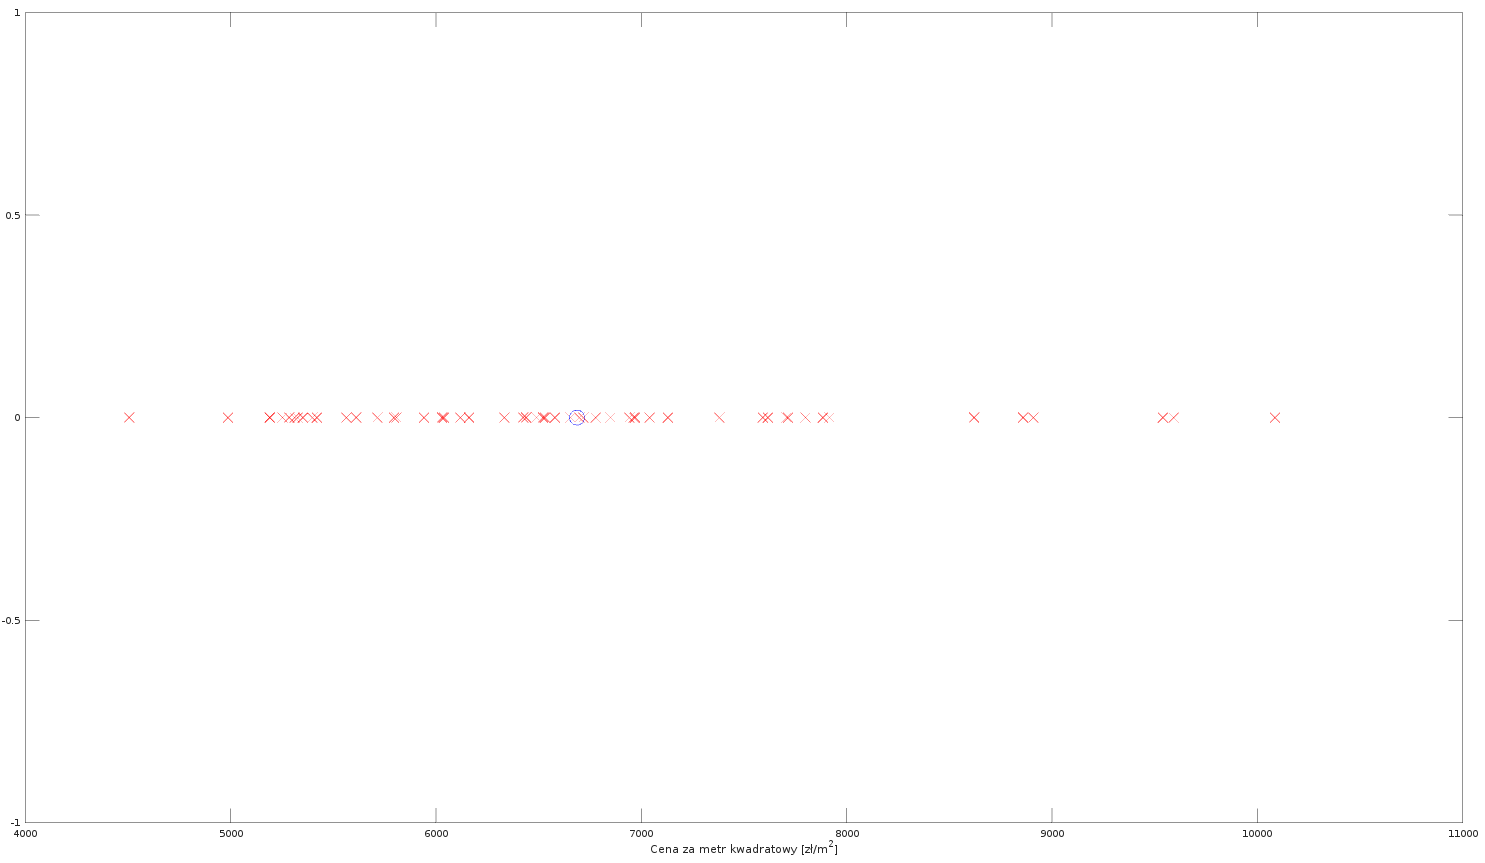
\includegraphics[scale=0.20]{PNG/1D.png}
    \caption{Wykres ceny metra kwadratowego dla wszystkich próbek}
    \label{lamana}
	\end{figure}
	

	\subsection{Dane po filtracji}
	
Jak widać filtracja odrzuciła nam trzy punkty maksymalnie po prawo. Nasz wykres został zmodyfikowany oraz te 3 próbki zostały usunięte z próbek, które będą używane podczas spadku gradientowego.\\


	\begin{figure}[H]
    \centering
    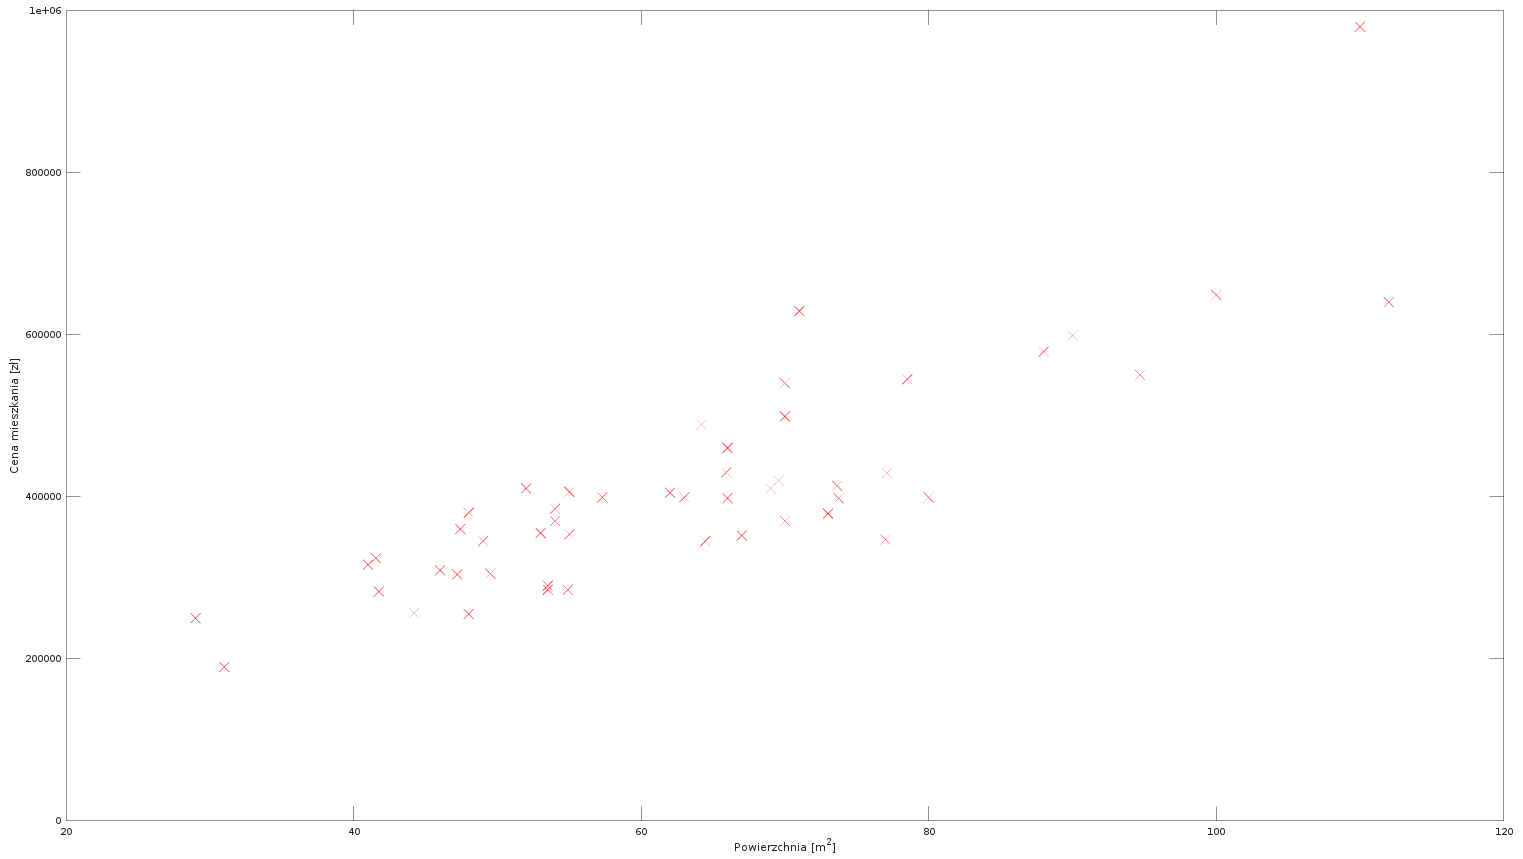
\includegraphics[scale=0.20]{PNG/y_X_filtracja.png}
    \caption{Wykres ceny metra kwadratowego dla wszystkich próbek}
    \label{lamana}
	\end{figure}
	

Po zobaczeniu nowego wykresu można zastanowiś się - czemu trzy punkty, które były skrajne i najbardziej oddalone od pozostałych nie zostały usunięte? To wszystko z powodu tego jaka była nasza filtracja - nie skupialiśmy się na punktach, które leżą najdalej od głównego skupiska punktów, a te których cena za metr kwadratowy jest najbardziej oddalona od średniej. Na przykładzie:
\newline
\noindent
Posiadamy cztery punkty i jeden z nich musimy odrzucić:
\begin{itemize}

  \item 100 metrów za 500 000 zł
  \item 60 metrów za 240 000 zł
  \item 50 metrów za 275 000 zł
  \item 40 metrów za 220 000 zł

\end{itemize}
\(
	z_{1} = 500 000 / 100 = 5 000 [zl] \\
	z_{2} = 240 000 / 60 = 4 000 [zl] \\
	z_{3} = 275 000 / 50 = 5 500 [zl] \\
	z_{4} = 220 000 / 40 = 5 500 [zl] \\
	s = (5 000 + 4 000 + 5 500 + 5 500) / 4 = 5 000 [zl] \\
	d_{1} = 0 [zl] \\
	d_{2} = 1 000 [zl] \\
	d_{3} = 500 [zl] \\
	d_{4} = 500 [zl] \\
\)
\newline
Jak widać na powyższym przykładzie odrzucona będzie wartość nie ta, która leży najdalej od reszty, gdybyśmy przedstawili ją na wykresie 2D, a ta której cena za metr kwadratowy najbardziej odbiega od średniej cen. Ważne jest by średnią cen za metr kwadratowych sporządzić na przykładzie cen z każdej próbki, a nie zsumować cenę wszystkich metrów kwadratowych oraz cen mieszkań - dzięki temu unikamy podwyższania ważności próbek, które posiadają wiekszy metraż.
\newline
\noindent
Dzięki filtracji pozbywamy się próbek, które mogą zaszkodzić naszemu algorytmowi. Zawsze warto zrobić filtrację danych, pod warunkiem, że będzie ona przemyślana i na pewno poprawna - dla przykładu trudno zrobić filtrację przy rozpoznawaniu cyfr, dlatego czasami lepiej warto ją ominąć i skupic się na samym algorytmie.